\section{Results}
In this section we test the proposed method on the models. The first idealized domain is a homogenous domain with shear wave velocity of $1000 km/s$. For more information about domain details and stations location see Fig.\ref{fig:3d_domain_scenarios}. Simulation record section shows a very clean arrivals (see Fig.\ref{fig:record_section_1000}.) We train the networks with 1000 set of input parameters. In this case we use PGV of north--south component in optimization process( results for other horizontal components or a combination of them are similar.)  We also generate a set of input parameters as a synthetic observation. The optimization algorithm search for parameters that are the best fit with synthetic observation.  Fig.~\ref{fig:station_1_1000_H1} shows the results of optimization process. For each station we repeat the optimization 50 times. We expect to see at each station, for the effective shear wave velocity (here \vs{}=1000~m/s), the optimized parameters and the target parameters $Q$ are very close to each other if not the same. 

  \begin{figure}[ht]
    \centering
    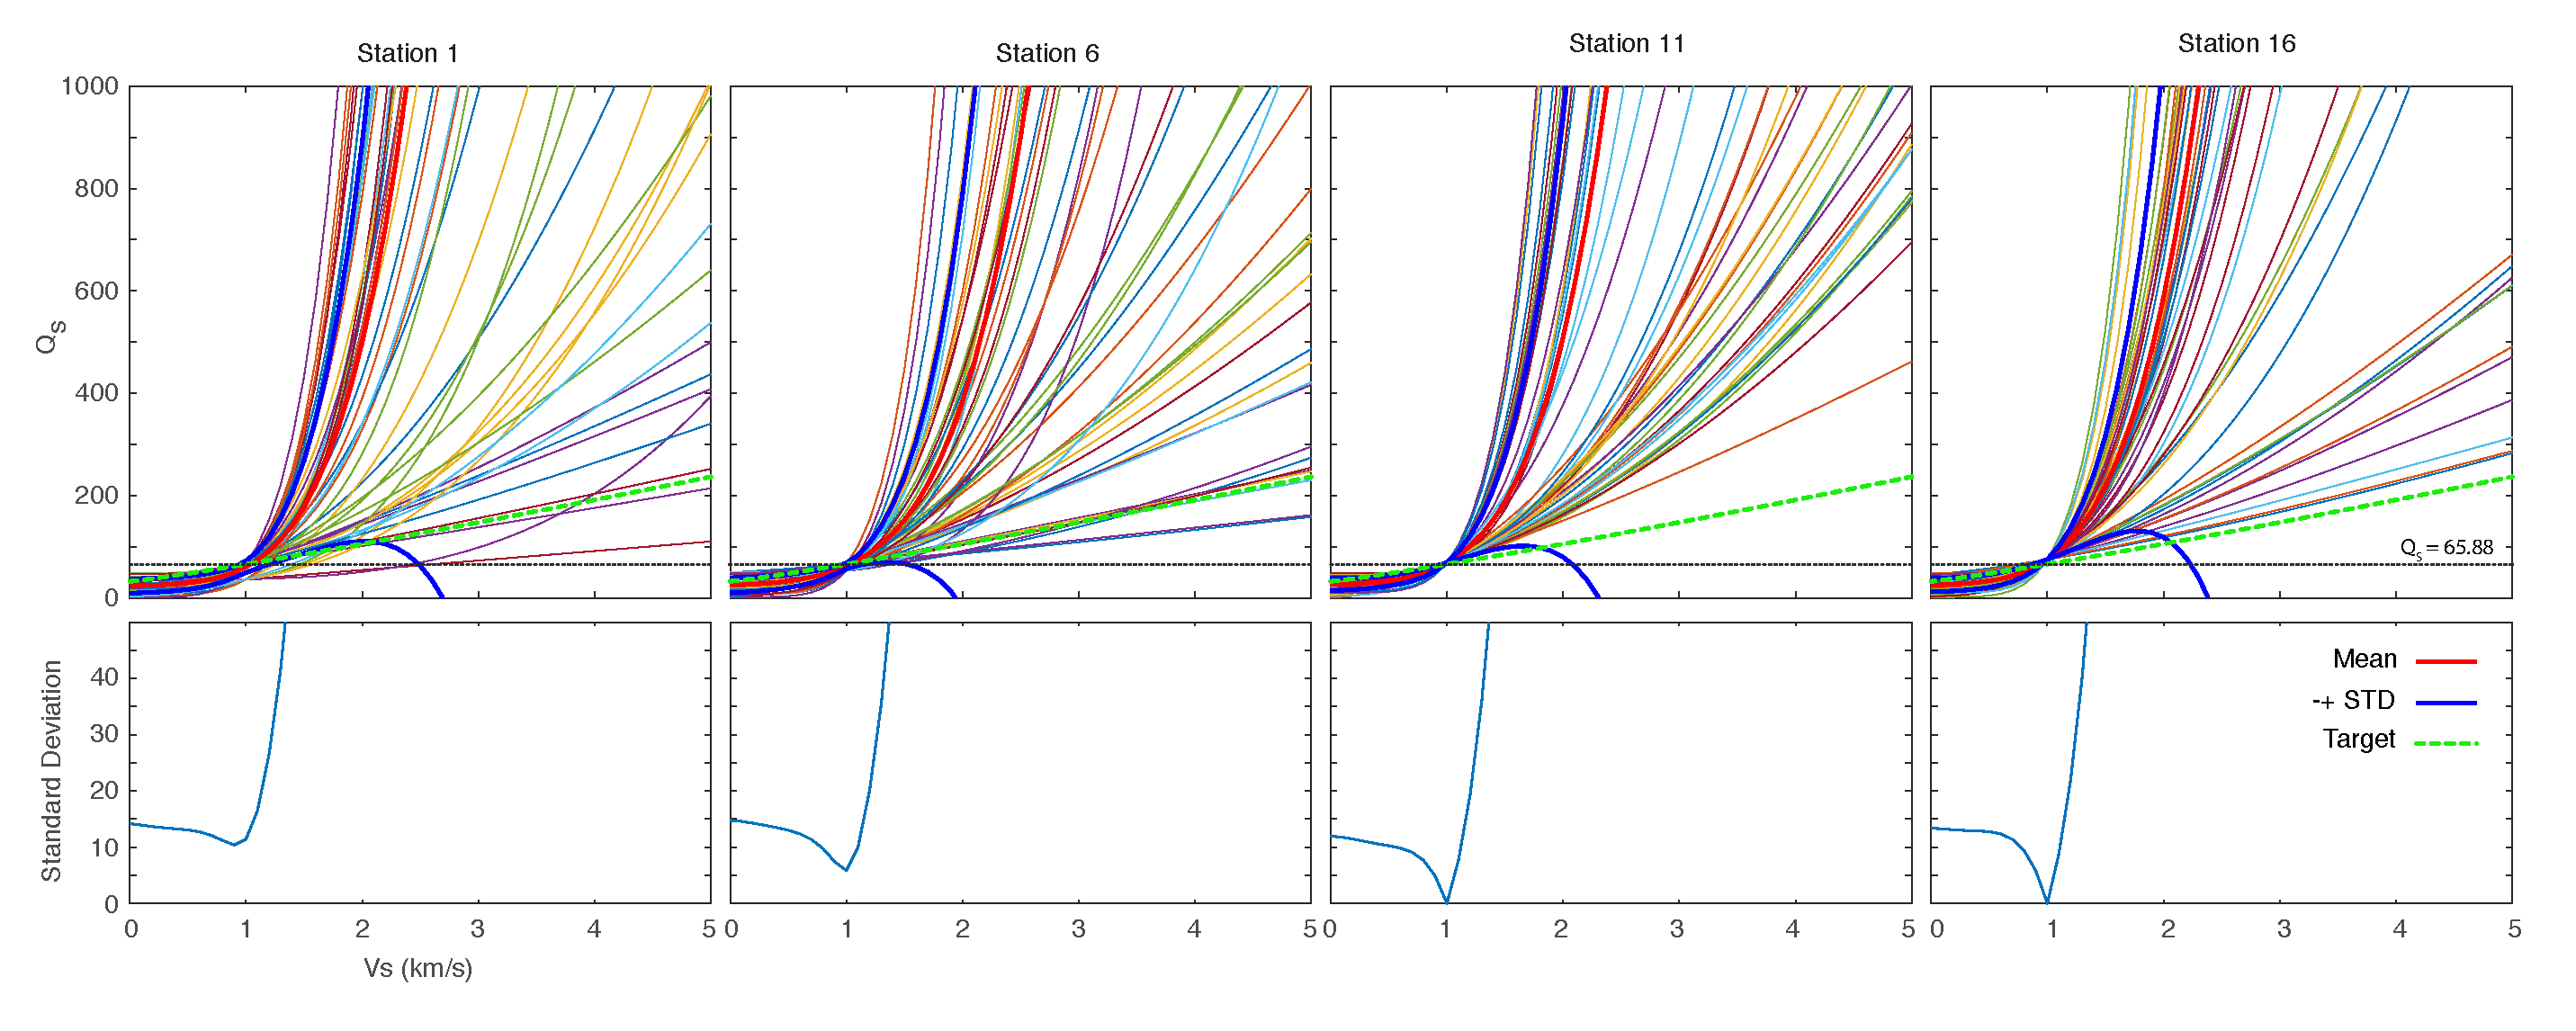
\includegraphics[width=\textwidth]{figures/pdf/Figure_14-H1-pgv.pdf}
    \caption{Results of 50 optimized solutions for homogeneous (H1) domain for 4 stations. The target simulation results are generated based on \qs{}$=32.17+33.71V_{S}^{1.12}$. In this simulation domain (\vs{}=1000~m/s), \qs{}=65.88}
    \label{fig:station_1_1000_H1}
\end{figure}

This figure shows stations 1,6,11, and 16. Standard deviation values which are shown at the bottom of the each stations are indications of convergence of the solutions. We expect to see a very small standard deviation at \vs{}=1000~m/s. Values of standard deviation is decreased at that \vs{}, however,  only station 11 and 16 have a very converged solutions. That is understandable, because at the closer stations the wave does not have chance to travel enough to capture the anelastic damping characteristics. The parameters that are used to generate the target values are shown with green thick dashed line. The convergence points are coincides with target value parameters at \vs{}=1000~m/s or is very close to it. This test gives the idea that for simple case if we can accurately pick the peak ground velocity, at considerable distance from the source, our optimization process can accurately estimate the $Q$ value for effective shear wave velocity by converging at that point. Also it can locate the $Q$ value with acceptable accuracy.
We add a shallow low velocity zone to the H1 domain. Fig.~\ref{fig:station_1_1000_500_L1} shows the results of optimization process. According to the results, as we observed in the homogeneous domain, the closes station to the source is not well converged, with increasing distance standard deviation decreases and also in mid-distance we can see effective shear wave velocity is in the range of 900--1000~m/s whereas at far stations with respect to the source the effective shear wave velocity is 1000~m/s. Obviously for far stations the wave are propagated more in the high velocity zone and are highly affected from that.   

  \begin{figure}[ht]
    \centering
    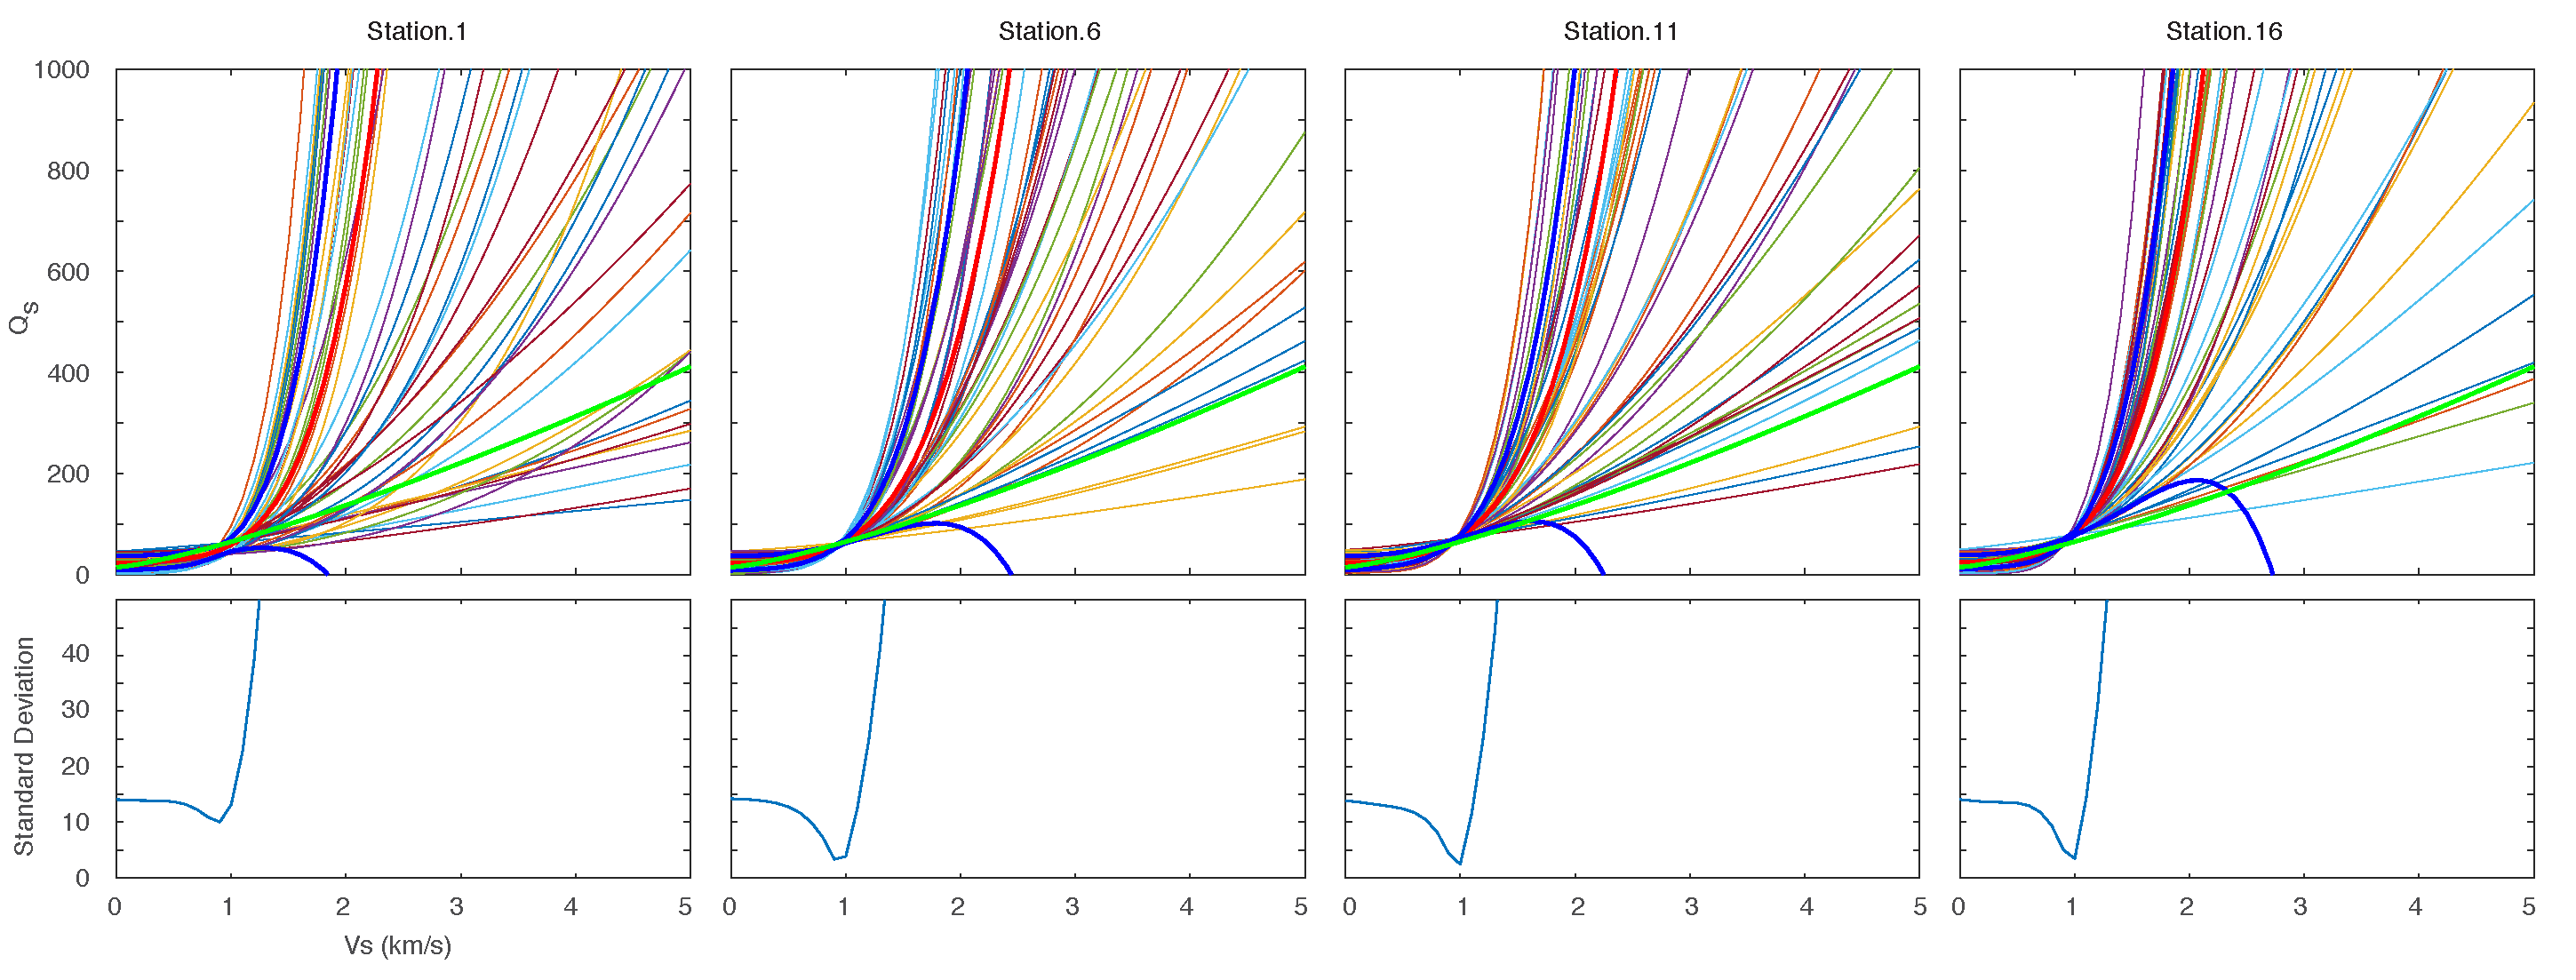
\includegraphics[width=\textwidth]{figures/pdf/Figure_15-L1-pgv.pdf}
    \caption{Results of 50 optimized solutions for Layered (L1) domain for 4 stations.  The target simulation results are generated based on \qs{}$=14.44+50.61V_{S}^{1.28}$. $Q_{S1000}$==65.05 is shown as a reference for \vs{}=1000~m/s}
    \label{fig:station_1_1000_500_L1}
\end{figure}

It is worth mentioning that effective shear wave velocity that is detected in this idealized scenario is not used in the simulation domain. However, the $Q$ value that is detected for that velocity coincides with the initial \qsvs{} relationship that is used.  The dashed green line is the parameters that we have used for developing synthetic observation values. Ideally, all stations, at their convergence point, should coincides with the line. Station 1 has a very weak convergence rate. Station 6, on the other hand, has a acceptable convergence in solution and also detect the initial parameters (dashed line). Station 11 and 16 have very sharp convergence, but the convergence point has a small difference with initial parameters $Q$ values. According to this results, we can say for this velocity and source model if we use PGV of north--south component as a determining metric, Station 6 most probably will detect the $Q$ parameters.
We increase the depth of low velocity zone of L1 domain (from 256 to 1024 m) to see if the effective shear wave velocities of each stations have considerable changes. Fig.~\ref{fig:station_1_1000_500_2_L2} shows the results of optimization process. The results show that the effective shear wave velocity becomes a little less than $1000~m/s$. It is understandable; because in this scenario the $500~m/s$ low velocity zone can have more effects on propagated waves. In this domain, Station 6 and 11 have good convergence and also could accurately detect the initial $Q$ parameters. 

  \begin{figure}[ht]
    \centering
    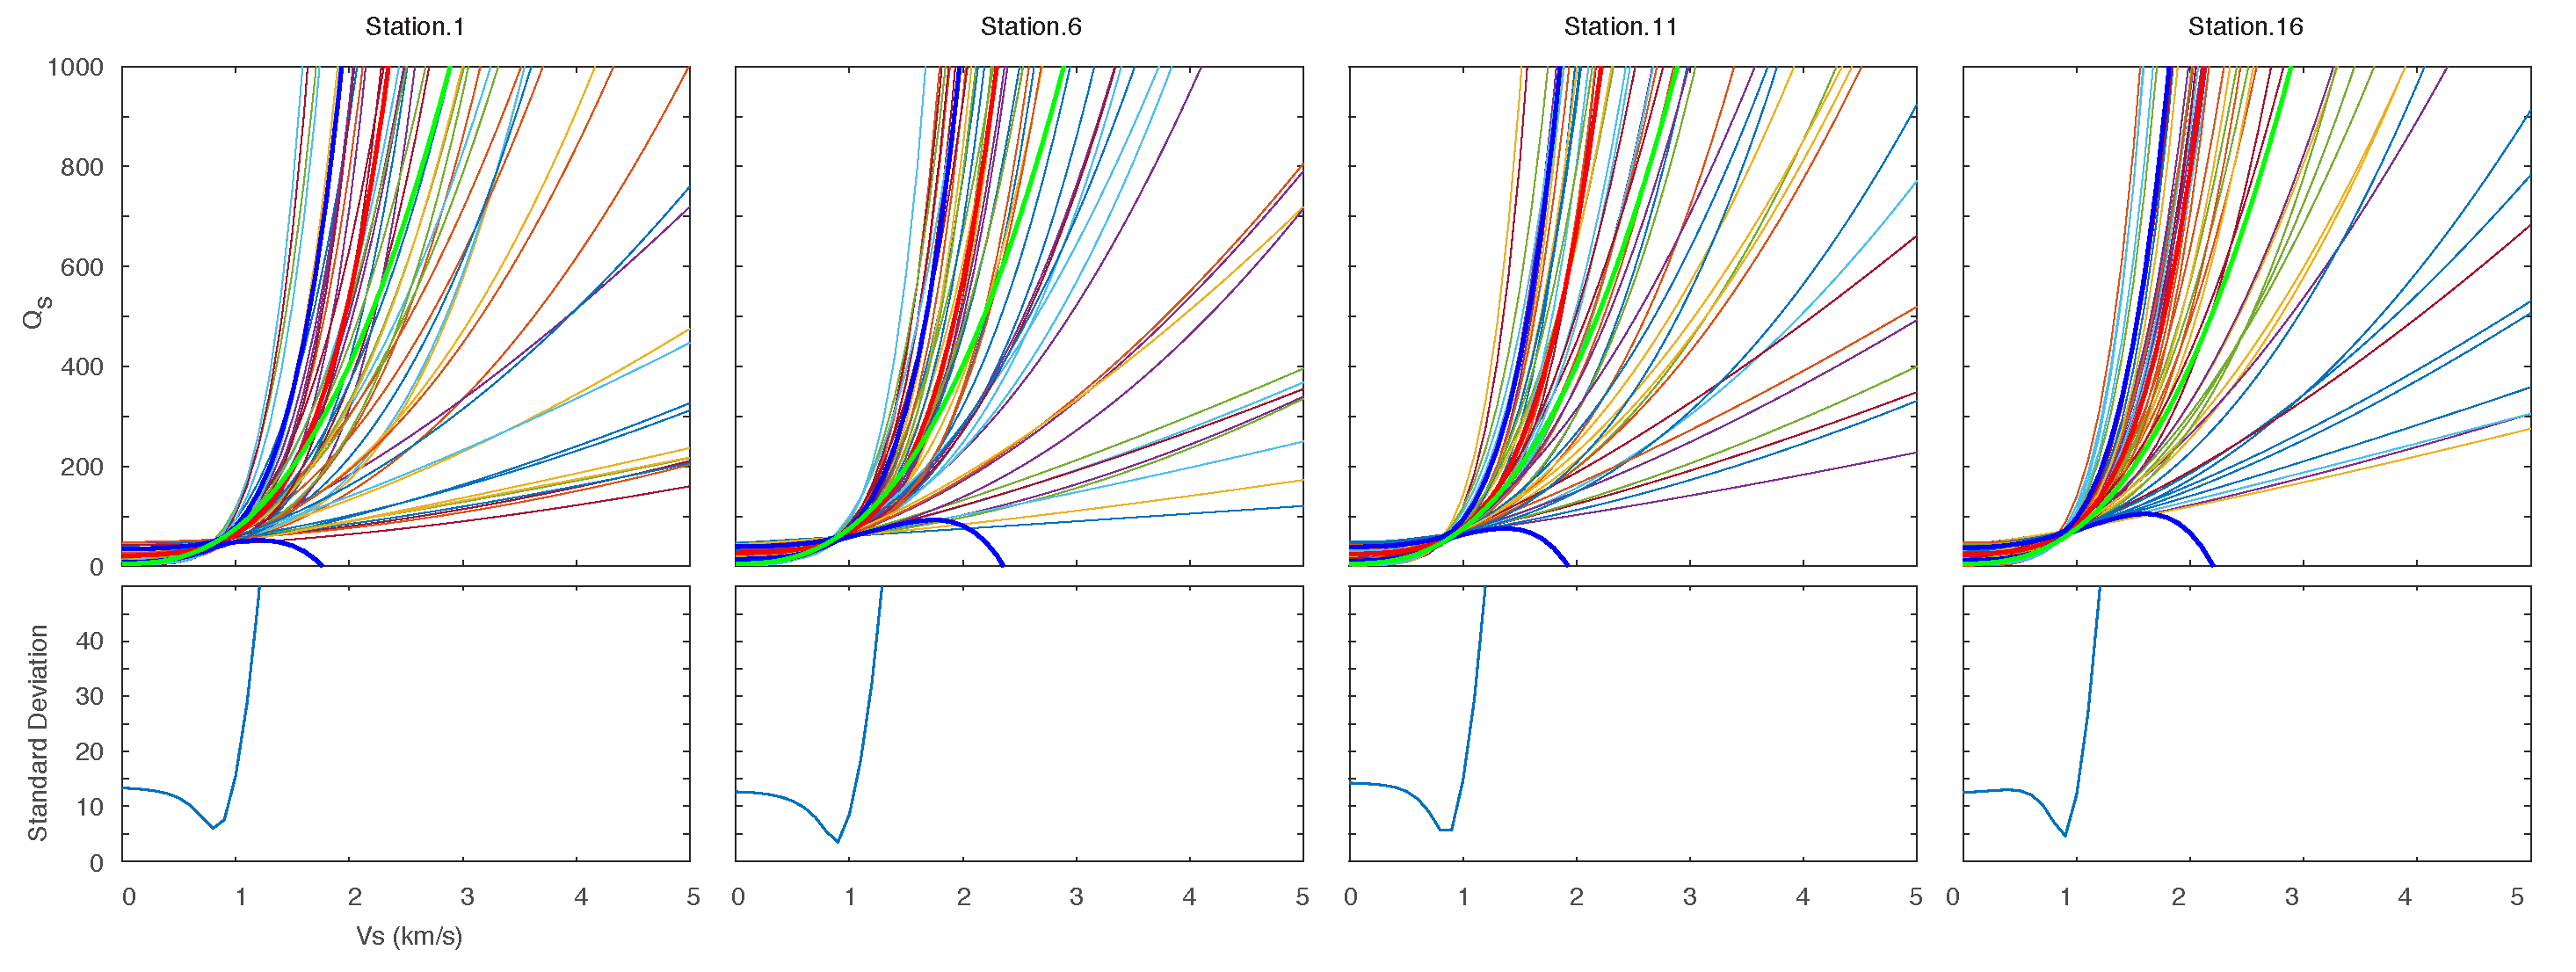
\includegraphics[width=\textwidth]{figures/pdf/Figure_16-L2-pgv.pdf}
    \caption{Results of 50 optimized solutions for Layered (L2) domain for 4 stations. The target simulation results are generated based on \qs{}$=5.21+70.11V_{S}^{2.50}$. $Q_{S1000}=$75.32 is shown as a reference for \vs{}$=$1000~m/s}
    \label{fig:station_1_1000_500_2_L2}
\end{figure}
 

We tried another idealized layered profile with three different layers. According to Fig.~\ref{fig:station_1_2000_1000_500_L3_nt}, with increasing distance from source (Station 1 to 16 ), effective shear wave velocity (i.e., minimum value of standard deviation) is shifting from lower velocity to higher velocity ( m/s to m/s). Far stations records are more affected with high velocity zone. 
 
  \begin{figure}[ht]
    \centering
    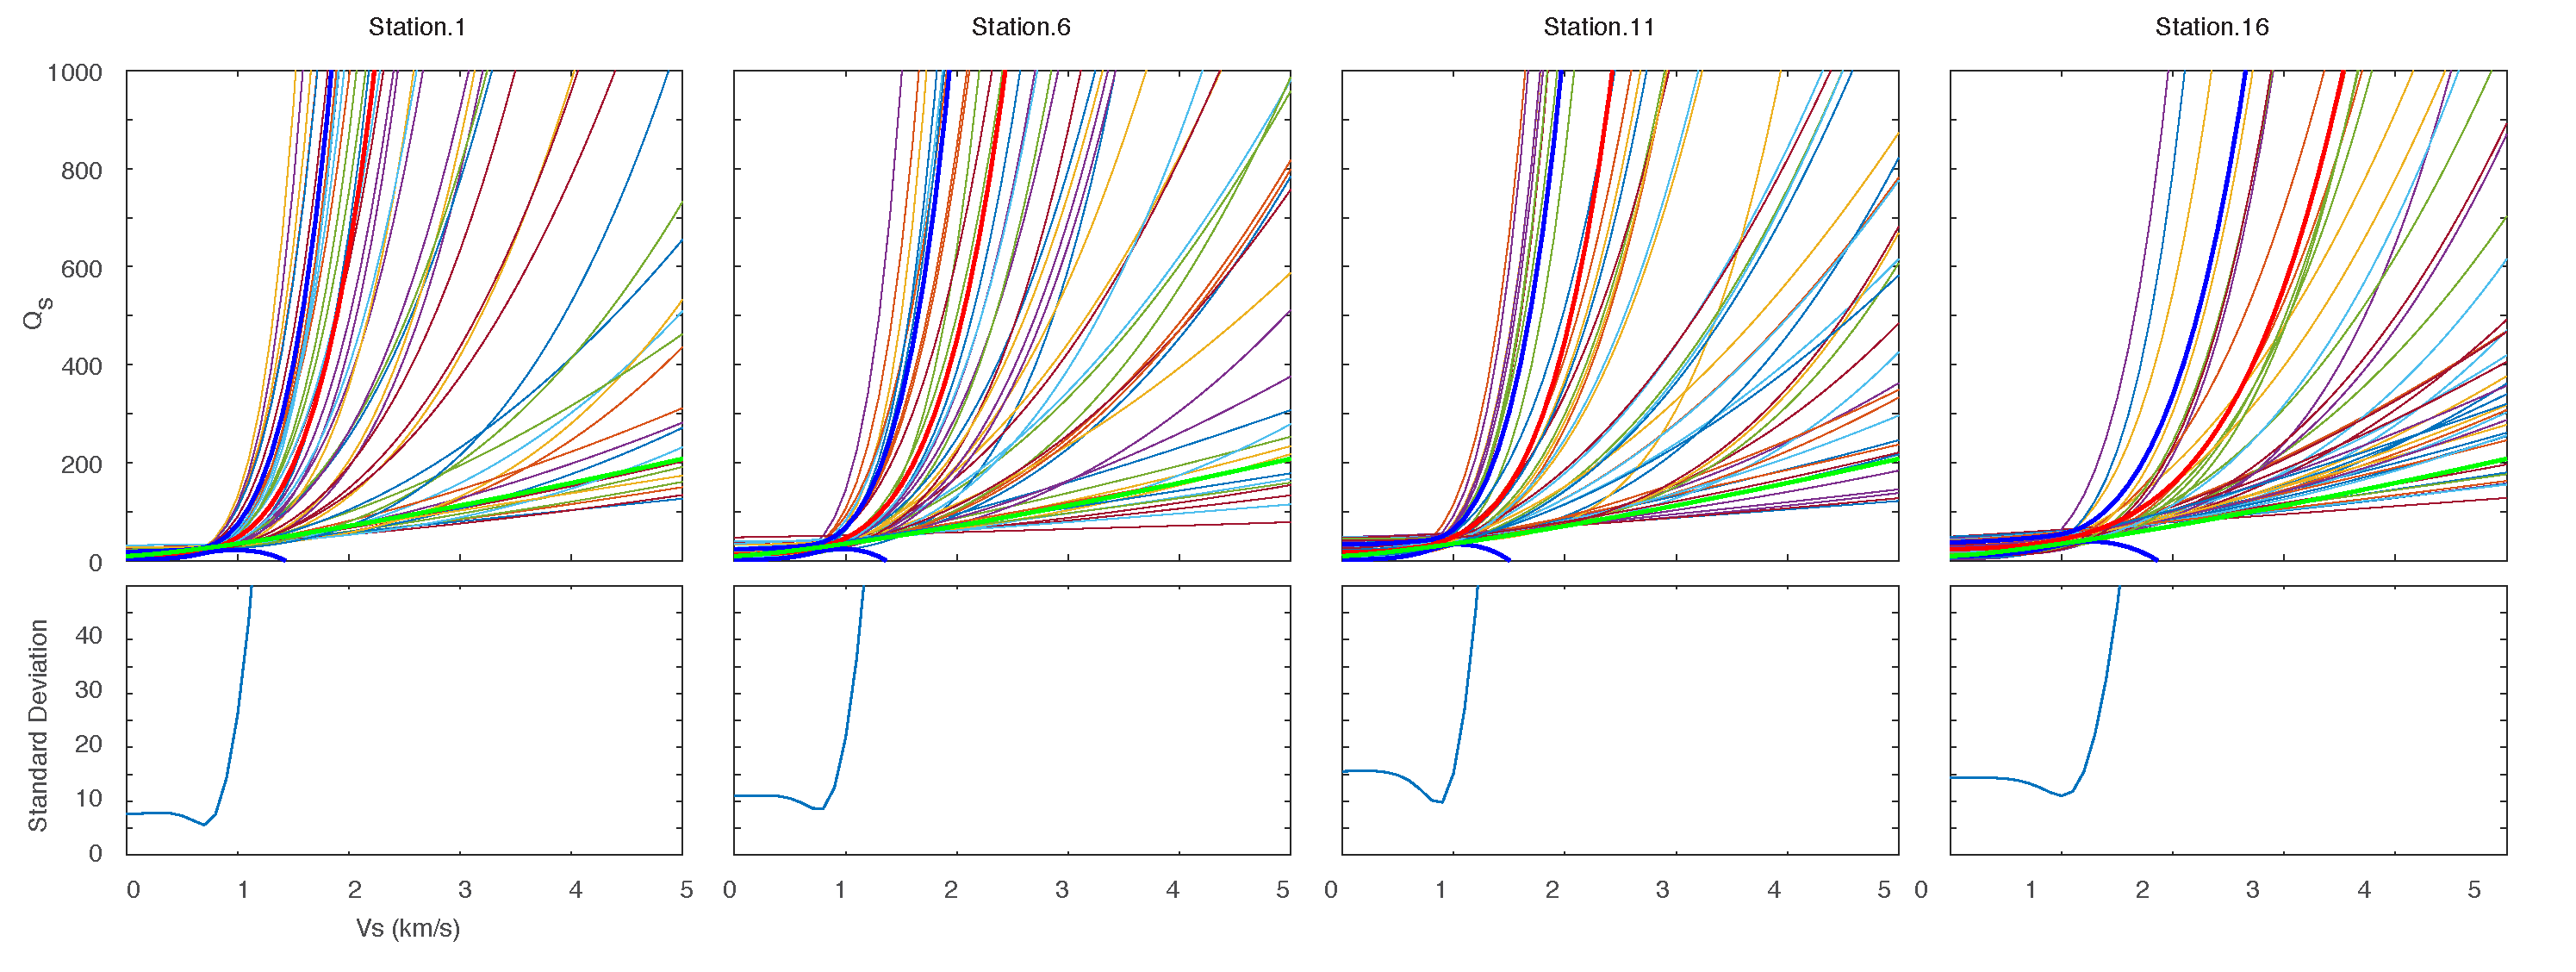
\includegraphics[width=\textwidth]{figures/pdf/Figure_17-L3-pgv.pdf}
    \caption{Results of 50 optimized solutions for Layered (L3) domain for 4 stations. The target simulation results are generated based on \qs{}$=9.28+25.31V_{S}^{1.28}$. $Q_{S1000}=$34.59 and $Q_{S2000}=$70.74 are shown as a reference for \vs{}=1000 and 2000~m/s, respectively}
    \label{fig:station_1_2000_1000_500_L3_nt}
\end{figure}

However, in this test, we do not see a good convergence rate. The standard deviation of the optimum results around the dominant shear wave velocity is slightly lower, but it is not as sharp as the simpler domains (e.g., H1). We achieved similar results for heterogeneous domain, as well. With increasing domain complexities, determination of effective shear wave velocity is not as sharp as before. It suggests that peak ground velocity may not be enough to estimate the results. Please note that the idealized scenarios do not have noise. Complex geological features (velocity models) make PGV less sensitive to input values. Therefore, we use the second ANN structure where it estimates PGV, PGA, SA1, and Venv for two horizontal components. Fig.~\ref{fig:station_8_param_2000_1000_500} shows the optimization results with using 8 metrics. 

  \begin{figure}[ht]
    \centering
    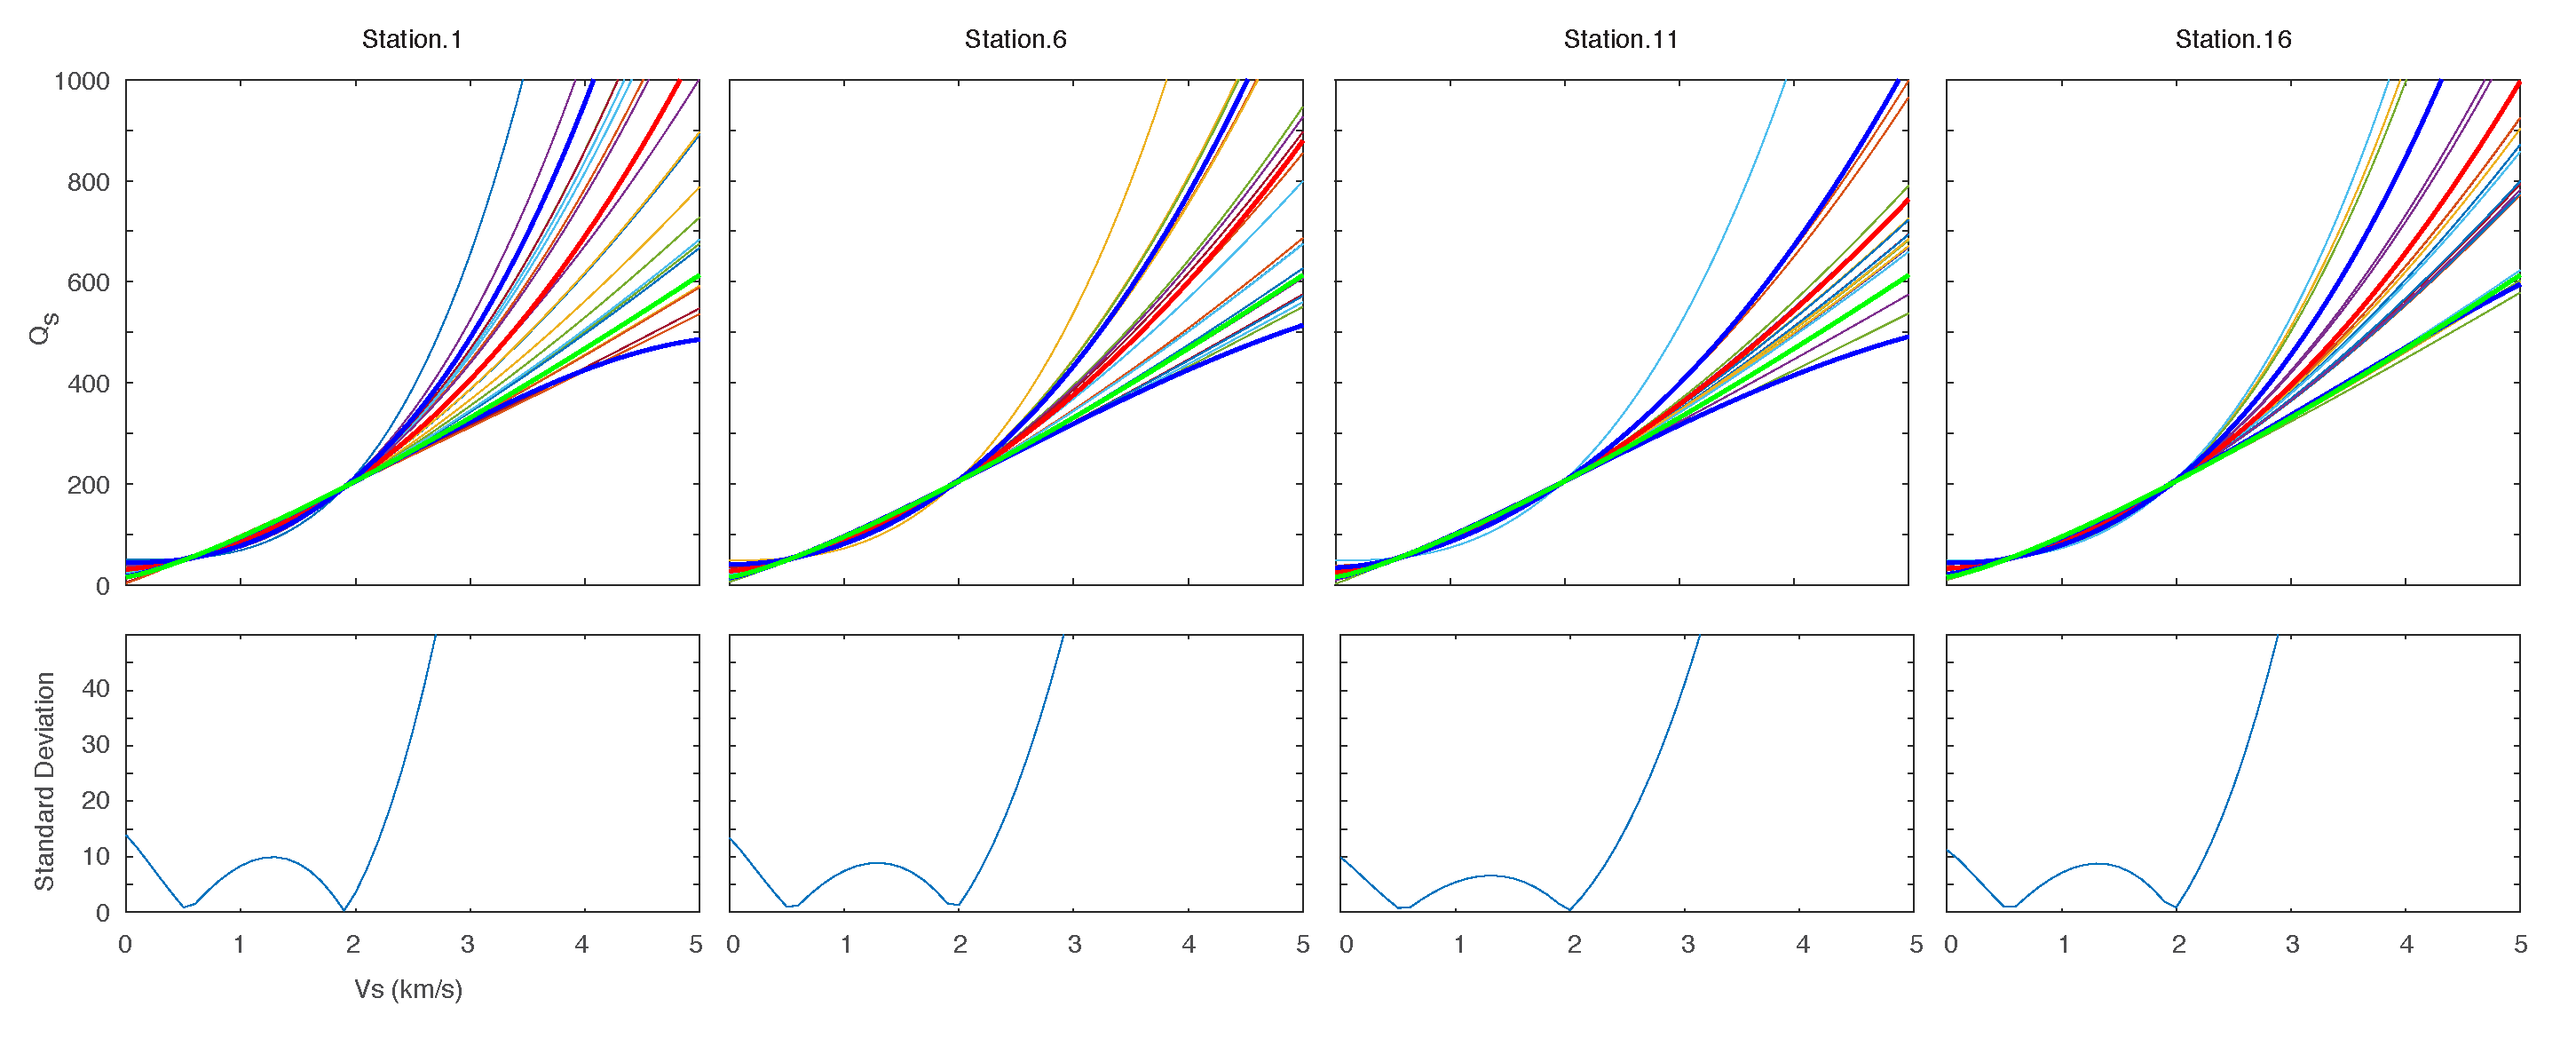
\includegraphics[width=\textwidth]{figures/pdf/Figure_18-L3-8metric.pdf}
    \caption{SA1, PGV, PGA, Env for NS and EW component. Domain(L3). The target simulation results are generated based on \qs{}=$15.12+80.00V_{S}^{1.25}$. $Q_{S500}=$48.76, $Q_{S1000}=$95.12, and $Q_{S2000}$=205.40 are shown as a reference for \vs{}=500, 1000, and 2000~m/s, respectively.}
    \label{fig:station_8_param_2000_1000_500}
\end{figure}

There is a significant improvement in the results. The algorithm can locate two ranges of effective shear wave velocities which are 500 and 2000~m/s in all stations. The results are not accurate for 1000~m/s. In this case, the current metrics and problem setup cannot retrieve valuable information for \vs{}=1000~m/s. This does not compromise the proposed method. The positive factor about the proposed method is that we know before hand that we cannot be confident about the results of \vs{}=1000~m/s. However, the results for \vs{}=500 and 2000~m/s are accurate. 
In idealized domains we show that the proposed method can locate a range of effective shear wave velocity and also accurately estimate the $Q$ values. Since idealized domains have up to three different soil layers. At the most elaborate case we will have three $Q$ values with respect to three effective shear wave velocity (in our examples we retrieved at most two effective shear wave velocity ranges.) We can fit a \qsvs{} relationship ($Q=C+\alpha V_{S}^\beta$) which will be similar to any of lines in Fig.~\ref{fig:station_8_param_2000_1000_500}. Obviously, we cannot expect to be able to acquire an accurate results for those shear wave velocity ranges that we have never used in the velocity model. For example in the case of L3 domain, we do not expect to be able to retrieve any accurate data for \vs{}=3000~m/s because the velocity model has 500, 1000, and 2000~m/s.  Therefore, in order to have a comprehensive results, we need to have more \qsvs{} points. In a heterogenous domain, with stations at different places and distance, we can retrieve many data points for different velocity ranges.
We use 2008  $Mw~5.4$ Chino Hills earthquake as a heterogenous domain platform to test the proposed method. The simulation domain and parameters are discussed in the Models Setup section. Fig.~\ref{fig:ANN_accuracy_stations_122_heterogenous_sim_177} shows the accuracy of the neural network for 8 output parameters for a station in the heterogenous medium. According to the figure and RMSE results, ANN can accurately be trained to estimate the requested metrics. We went through all stations, and almost all of them are similar to this station results. Please note that the 50 test data which are used here have never been seen with algorithm during the training session. This figure shows that, only second test data, at one or some ANNs, have slightly different results than actual observation. We can say that based on the red crosses that are obvious above and below the actual value (blue circle) of the second test data.   

  \begin{figure}[ht]
    \centering
    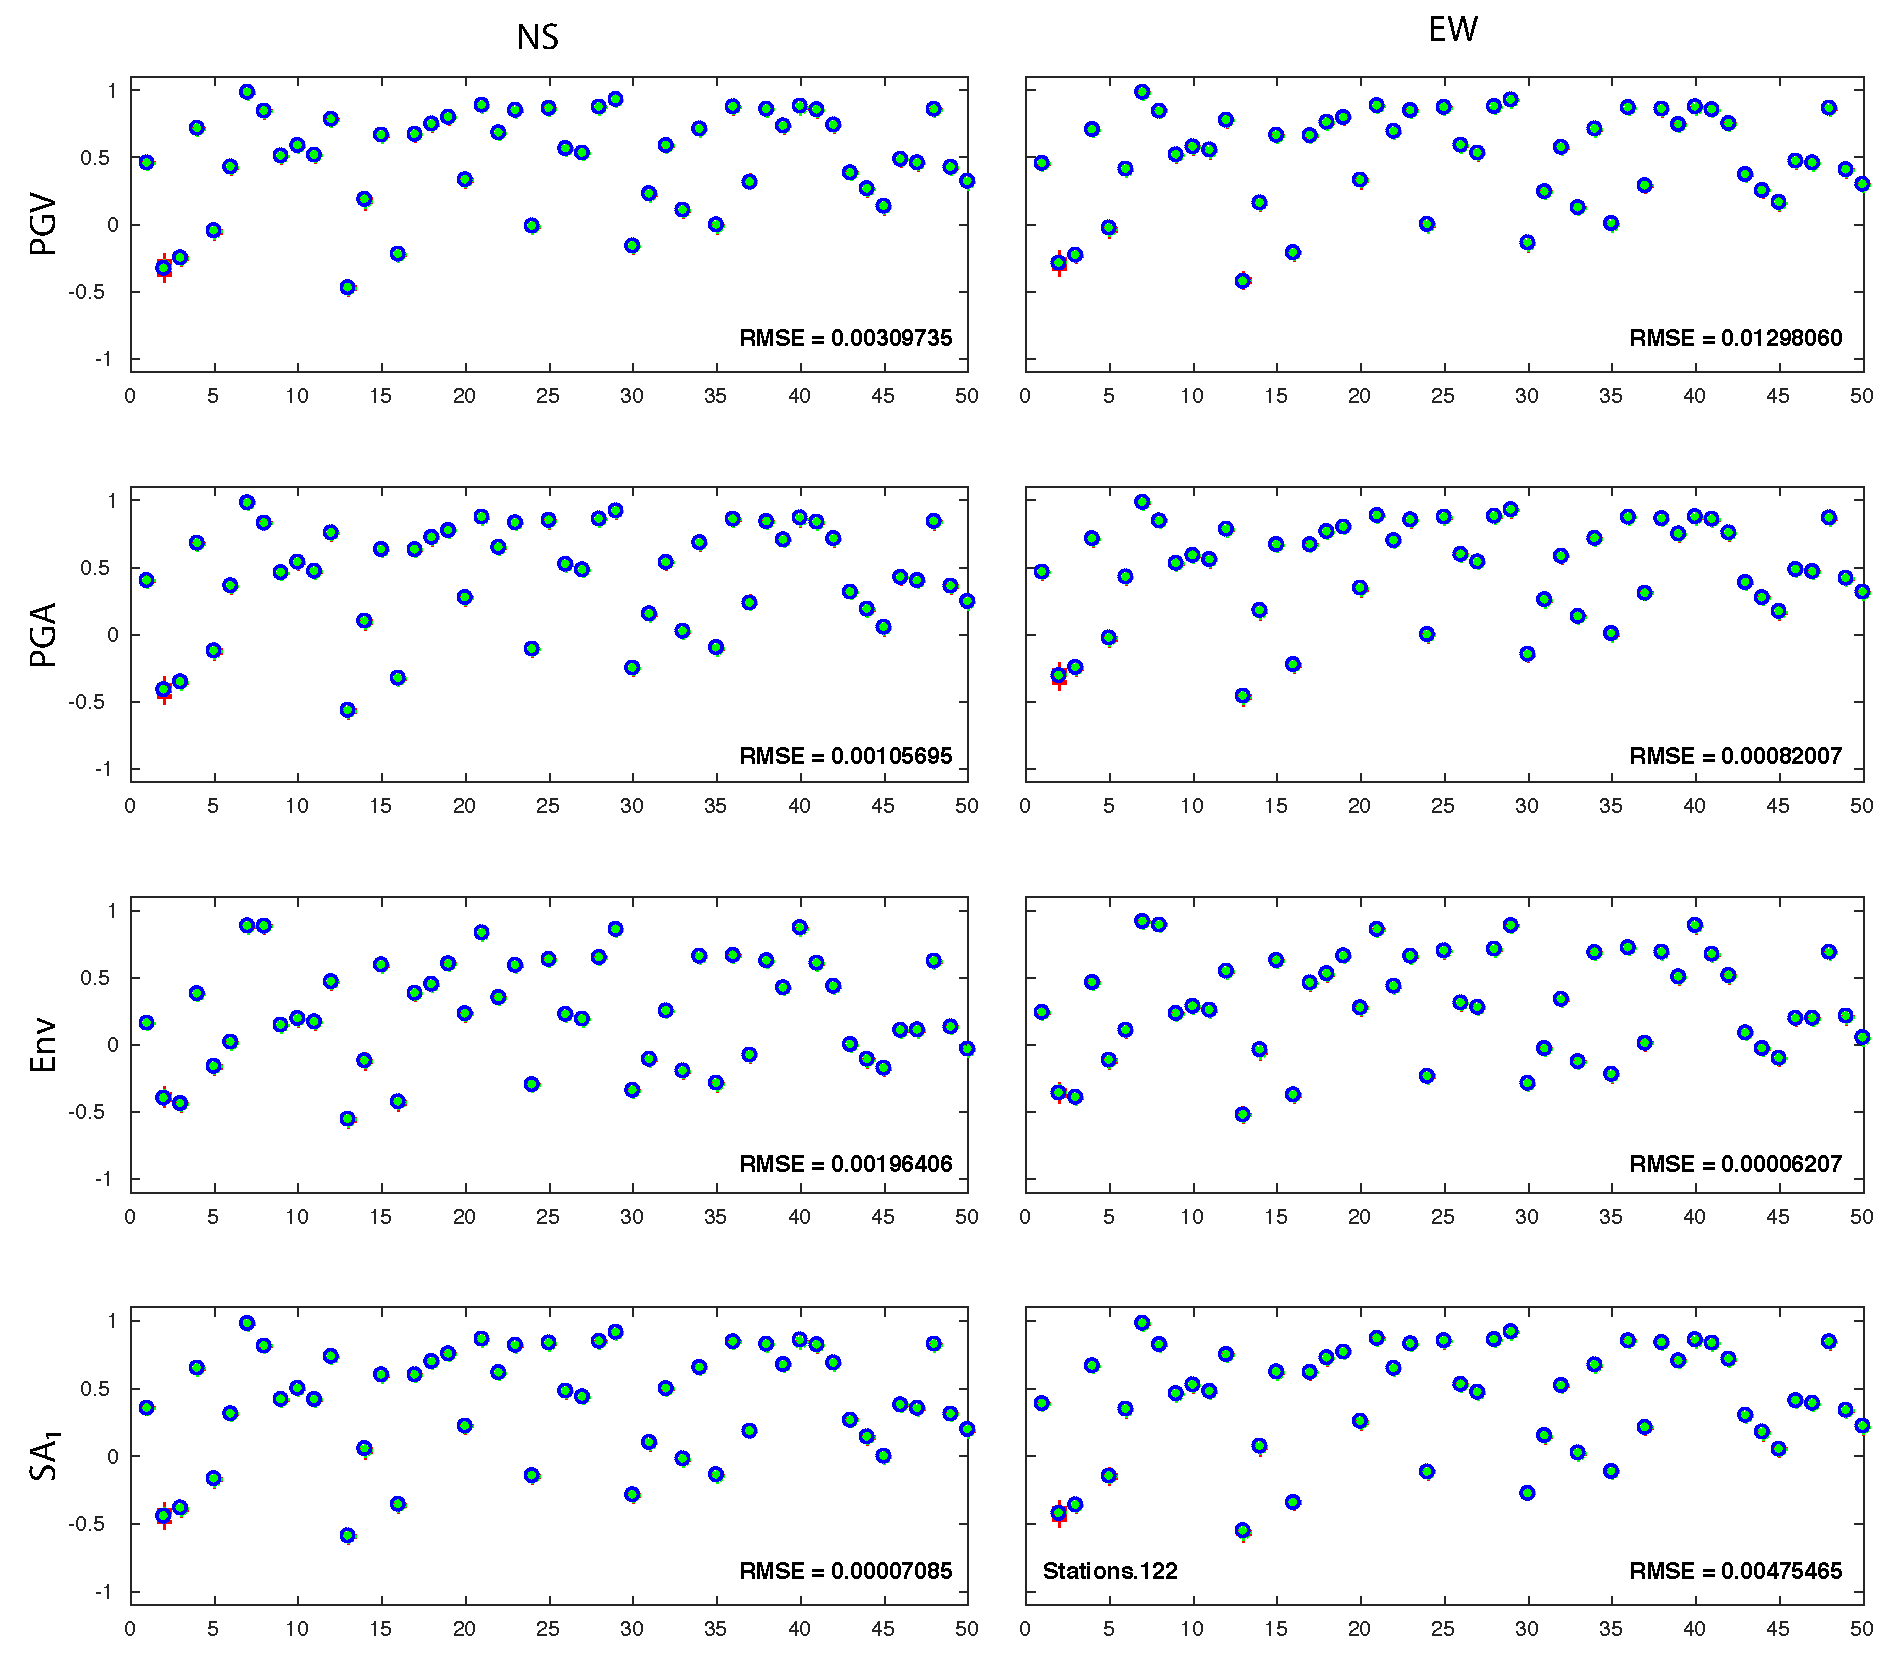
\includegraphics[width=\textwidth]{figures/pdf/Figure_19-st122_het_sim_177.pdf}
    \caption{Accuracy of the results for station number 122 in the heterogenous domain. The station is located in about 42 km from the source (hypo central distance).  }
    \label{fig:ANN_accuracy_stations_122_heterogenous_sim_177}
\end{figure}
 
We follow the steps that we explained at methodology section. We compute the mean of 50 optimized $Q$ values and find the closest $Q$ equation in the training data. We run the optimization process for estimating the new test value which is very close to observation. This process helps us to understand whether the optimization process can find the actual results where we know the input parameters before hand and is very close to the potential field parameters. Those data which pass the following checklist are added to the final Qs-Vs dataset. The criteria is according below:

\begin{itemize}
\item If synthetic solution is converged for a range of shear wave velocity (Standard deviation is an indication of this situation)
\item If the optimizaiotn process successfully locate the input parameters
\end{itemize}

After passing these steps, we generate a dataset and compute another regression analysis to estimate the \qsvs{} relationship that fits the data. As we can see from idealized domains, not all stations and metrics are equally good in extracting all velocity information. This fact also happens in heterogenous domain with fairly complicated source model. Fig.~\ref{fig:used_stations_example} shows four stations that some velocity range of them can pass the defined criteria. 

  \begin{figure}[ht]
    \centering
    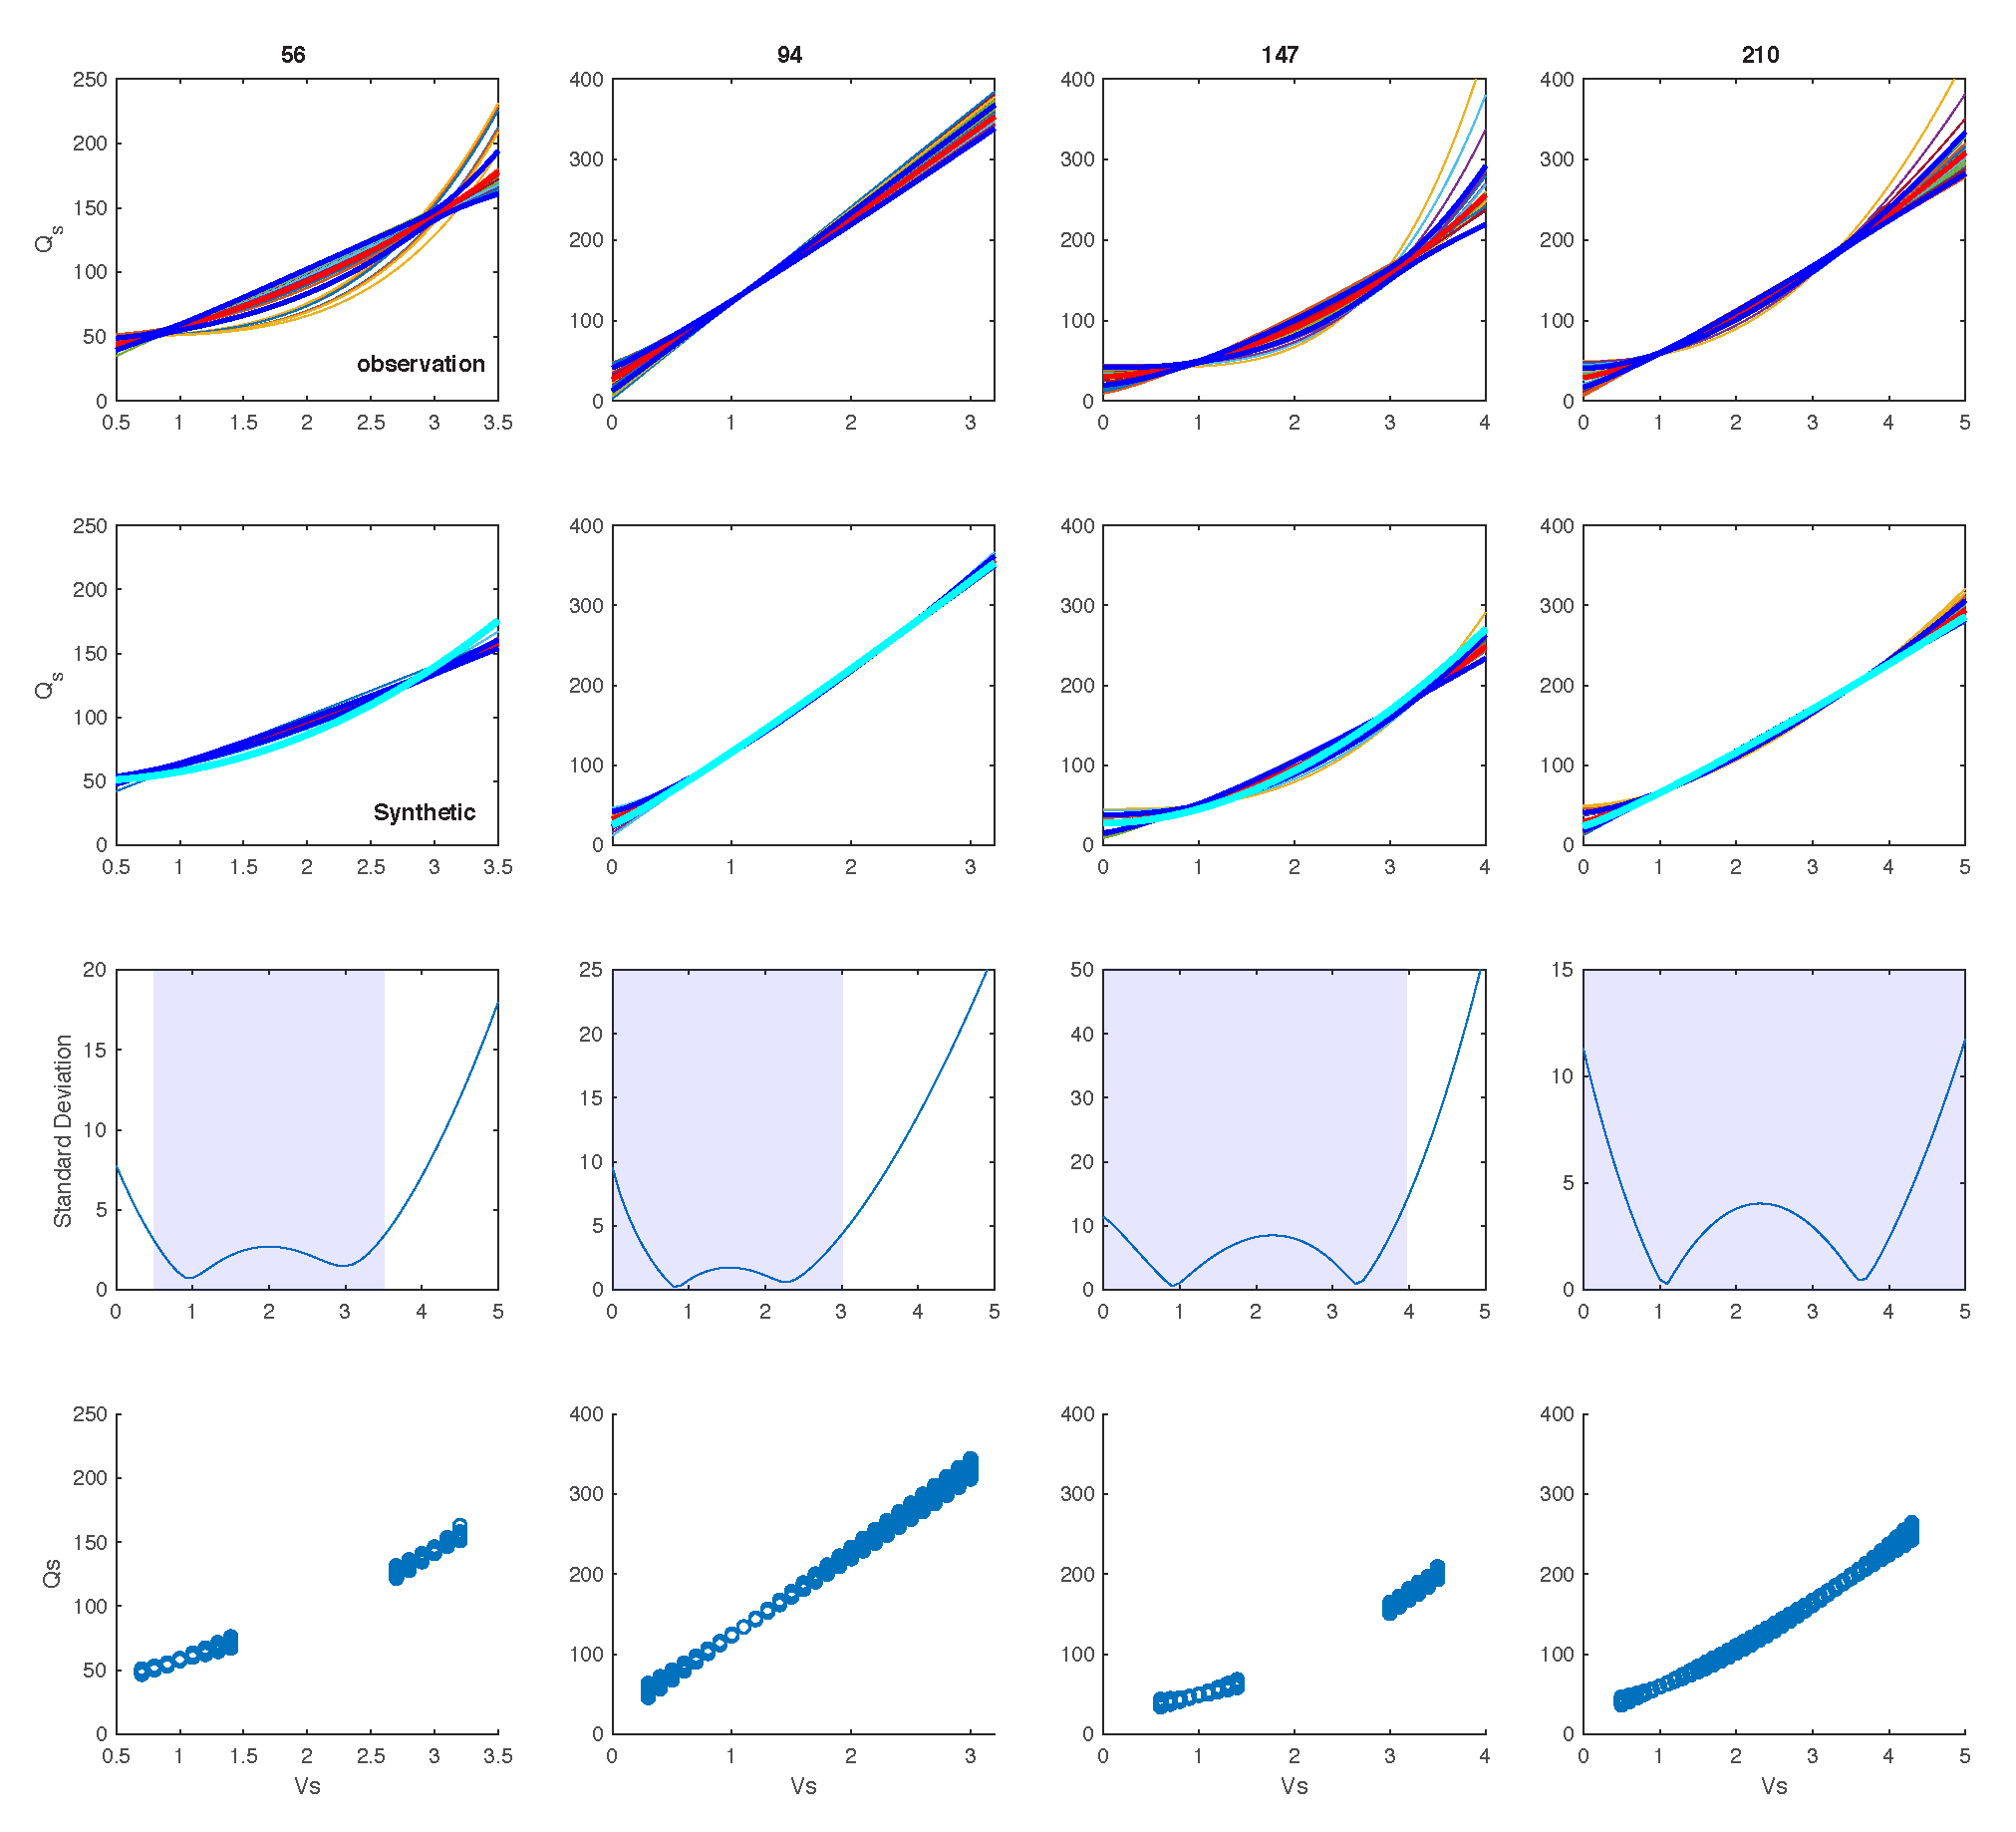
\includegraphics[width=\textwidth]{figures/pdf/Figure_20.pdf}
    \caption{Some of stations in the heterogeneous domain that pass the criteria. The cyan line in synthetic represent the closest available data in training dataset.}
    \label{fig:used_stations_example}
\end{figure}

These four stations are example of stations that part of their shear wave velocity range are used in the final analyses. Each station provides enough information for different range of shear wave velocity. The observation and synthetic are converged at fairly close shear wave velocity ranges for both observation and synthetic. Also in those ranges the algorithm can successfully retrieve the $Q$ value parameters that is used as an input for synthetic target value. The mentioned criteria are met and we can use the results of observation in that range. In order to choose more conservative values for each appropriate shear wave velocity we use only those data that are between $\pm$ standard deviation lines. In all figures these lines are shown using thick blue lines. Similar to the idealized cases, there are stations that cannot pass the defined criteria. Figure.~\ref{fig:unused_stations_example} shows some of these stations. 

  \begin{figure}[ht]
    \centering
    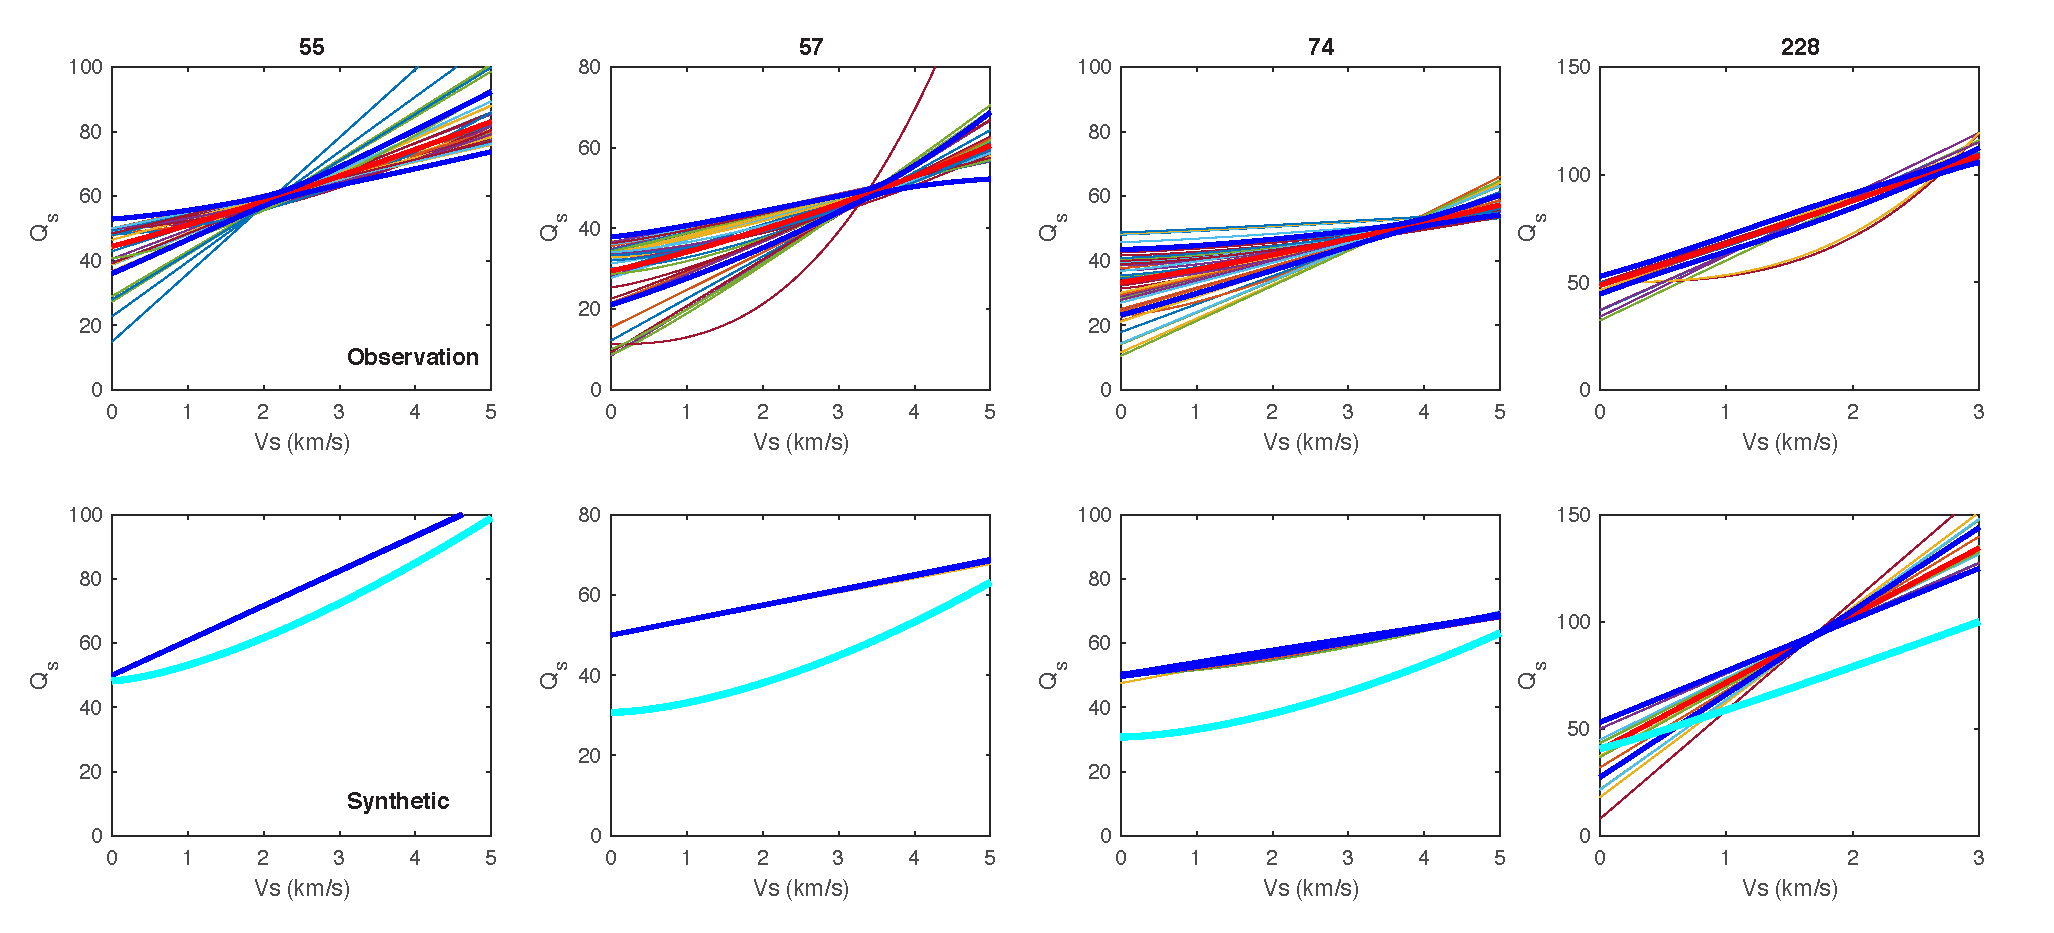
\includegraphics[width=\textwidth]{figures/pdf/Figure_21.pdf}
    \caption{Some of stations in the heterogeneous domain that fails the criteria. }
    \label{fig:unused_stations_example}
\end{figure}

Stations that are represented in Figure.~\ref{fig:unused_stations_example} are not used at the final process. The optimization algorithm provides very converged results at least for three of these stations. However, none of these results are according to the input parameters for target values (dashed green line). This suggests that these stations are not trustable to estimate the observation values. Without the synthetic section of the analyses one arguably can use the converged results of observation. However, the figure shows that the converged $Q$ values are not coincides with initially used $Q$ values. There is a possibility that signal metrics are not conclusive enough to capture the input parameters. The results show that the proposed steps can lead to very accurate and confident parameters. 
The final dataset which we believe is the most appropriate information that we can extract from our dataset in shown in the Fig.~\ref{fig:results_conservative_with_regression} . We use opacity filter and jitter to provide an estimation about the density of points in the figure. In computing the final equation for the Q factor, we ignore data with shear wave velocity less than 350 m/s according to minimum shear wave velocity of the simulations. We use GA optimization to search for the best \qsvs{} relationship that fits dataset.  The final result is $Q_{S}=7.1+60.2 V_{S}^{1.00}$. 


  \begin{figure}[ht]
    \centering
    \includegraphics[width=\textwidth]{figures/pdf/Figure_22.png}
    \caption{Scatter data of stations which passed the optimization criteria. Left: Actual data. Different colors represent different stations. Right: Same data with jitter and opacity filter to represent the data density and distribution.}
    \label{fig:results_conservative_with_regression}
\end{figure}





% The proposed method can retrieve two 

% We can argue that there should not be any problem with optimization process.  

%The idea of effective shear wave velocity or average shear wave velocity is not a novel concept. It is used in many different application to estimate the overall shear wave velocity of a soil profile (e.g., see time average method for shear wave velocity in geotechnical engineering applications).  

